% !TEX root = ../msc_thesis.tex

\chapter{Results}
\label{cha:results}
To the extent of our knowledge and research, no prior work exists that examines strength meters in a partial password setting. The results of our research are therefore the first ones published for this setting and can serve as a baseline for future research on the subject. At the same time, we can indirectly compare our findings with the ones from research on traditional passwords, and examine if some hypotheses hold true in both settings.

The primary goal of this research was to examine the effect of the partial password meter on the strength of the created partial passwords, and secondly, its effect on their memorability. In order to draw conclusions, we formulated and tested the following null hypotheses in the field:

\begin{itemize}
  \item[] $H_{0a}$: Partial passwords are not stronger when the partial password meter is present during creation.
  \item[] $H_{0b}$: Partial passwords are not more memorable when the partial password meter is present during creation.
\end{itemize}

Following the same methodology as Ur et al., we conducted an online study consisting of two parts. Ideally, the study would be conducted with participants that were using partial passwords in their online routine - possibly limiting the demographic to UK residents. An option to gather the necessary data would be to run the experiment in an on-campus laboratory environment, recruiting students and other researchers to participate in the study. We deemed that doing so would restrict us to a very specific demographic, with a distinct age distribution, education level and experience in research studies and could therefore skew the results. In order to align this research as best as possible with previous work, a crowdsourcing platform that uses a mainly UK demographic and on which custom Human Intelligence Tasks can be specified for execution would be an ideal solution. Unfortunately, after examining the available options, none was found that fit the criteria, while also being cost-efficient. Ultimately, we decided recruiting subjects for our study (also referred to as \emph{workers}) from Amazon's MTurk platform, while providing them with a brief introduction and explanation of partial passwords.

Participants were required to be at least 18 years old and use a web browser with enabled JavaScript capabilities. The details for each task are described in the following sections. While not directly mentioning the purpose of the study to the subjects, we did not employ subterfuge to hide it, unlike what Egelman et al. did in their study~\cite{strength_meter_impact}. By saying that ``We are conducting an academic survey about partial challenges on passwords and we are testing a new partial password system.'', participants were made aware of the general focus of this research. Since we were particularly interested in accurately pinpointing the effect the password meter had in the strength of the created passwords, we decided to use a significance level of $\alpha = 0.01$ for that statistical test, in order to minimise the probability of a type I (false positive) error. For all other statistical tests in our analysis, the common $\alpha = 0.05$ value was used.


\section{Empirical evaluation of partial strength metric}
  \label{sec:correctness}
  Before setting out to test the hypotheses, the correctness of the implemented partial password meter needed to be verified. As mentioned in Section~\ref{sec:str_meter_existing}, the term ``password strength'' is ill-defined, which renders a theoretical proof of correctness impossible. In accordance with the definition of password strength we adopted, a practical approach was followed when testing the correctness of the developed meter.

  A Python script containing the partial password strength calculation algorithm described in Section~\ref{ssec:str_metric} combined with a projection dictionary generated by the RockYou dataset was used to evaluate the password strength of different password lists. The password lists tested were the password database leaks from the RockYou website and the PHPBB forums, as well as the top 10 million passwords dictionary released in 2015~\cite{top10m_pass}, a revision of the top-500~\cite{top500_pass} and top-10000~\cite{top10000_pass} password lists released in 2005 and 2011, respectively. For each set, we filtered out the passwords that did not meet the specified length (6-15 characters) and discovered the most common password that was ranked as ``Strong'' or ``Very Strong'' from our algorithm. The Python CLI version of the strength meter was used for faster and more flexible offline evaluation of the aforementioned dictionaries - the algorithm and scores are consistent between the Python and JS implementations.

  The findings of the aforementioned analysis are displayed in Table~\ref{tab:str_correct}. We observe that the algorithm is adequately strict in the ranking of partial passwords, even when testing other datasets. It is worth noting, that while these passwords seem and are weak in a traditional setting with offline dictionary attacks, the chance of successfully guessing a partial password challenge of them within $\beta = 10$ max guesses in an online attack scenario is minuscule. We conclude therefore that the strength metric's performance is acceptable and can be used to test the selected hypotheses.

  \begin{table}[htpb]
    \centering
    \small
    \hspace*{-1.5cm}
    \begin{tabular}{|c||c|c|c|c|c|c|}
      \hline
      \textbf{Dataset} & \multicolumn{2}{|c|}{\textbf{RockYou}} & \multicolumn{2}{|c|}{\textbf{PHPBB}} & \multicolumn{2}{|c|}{\textbf{top 10M}} \\
      \hline
      \textbf{Verdict} & \textbf{Strong} & \textbf{Very Strong} & \textbf{Strong} & \textbf{Very Strong} & \textbf{Strong} & \textbf{Very Strong} \\
      \hline
      \textbf{\# of passwords} & \multicolumn{2}{|c|}{31063584} & \multicolumn{2}{|c|}{230905} & \multicolumn{2}{|c|}{9061038} \\ \hline
      \textbf{Most common} & \multicolumn{2}{|c|}{50cent} & \multicolumn{2}{|c|}{qazwsx} & 696969 & 1qaz2wsx \\ \hline
      \textbf{Frequency} & \multicolumn{2}{|c|}{3294} & \multicolumn{2}{|c|}{92} & 3050 & 2531 \\ \hline
      \textbf{\% frequency} & \multicolumn{2}{|c|}{0.011\%} & \multicolumn{2}{|c|}{0.040\%} & 0.034\% & 0.028\% \\ \hline
    \end{tabular}
    \caption{Most common password ranked ``Strong'' or ``Very Strong'' per dataset}
    \label{tab:str_correct}
  \end{table}


\section{Effect on partial password strength}
  \label{sec:usability}

  \subsection{Methodology}
    \label{ssec:usability_setup}
    We recruited 200 participants from Amazon MTurk to participate in this research. For the first part of the study, subjects were paid 75 cents and were asked to ``Answer a survey about partial passwords after completing a mock registration process''. In order to qualify for the task, they had to complete a small screener test that ensured they were able to correctly answer partial password challenges. This qualification test also served to prime workers for the task and inform them about the concept of partial passwords, since most of them were expected to not have experience with partial password login systems, as our prior survey indicated (described in Section~\ref{sssec:partial_pass_extent_use}). Before the task was published, a small-scale (20 subjects, both MTurk workers and university students) pilot was carried out, in order to discover possible bugs or other problems with the website. Since the feedback received from this pilot run motivated changes in the website and the strength meter, we discarded their results to ensure consistency within the study samples. The participants in our study were heavily based in the US (183/200, 91.5\%), and had a 60/40 Men/Women ratio. Ages varied from 18-69, having a mean age of 32.77 with 10.07 standard deviation and with 46.5\% of the participants being in the 26-35 age range.

    Participants were randomly assigned to either the control or the experiment condition and were asked to complete a registration process on our website, followed by a successful login using a partial challenge on their passwords, as shown in the control flow in Figure~\ref{fig:control_flow}. After successfully logging in, they were presented with a survey containing questions about their opinions concerning the strength meter (this group of questions differed between conditions), questions about the partial password and their method of answering the challenge, as well as some basic demographic questions. The multiple-choice survey questions were presented in a equidistant (neutral) manner and designed to offer five-level Likert-type scale responses~\cite{likert}, in order to minimise user bias. An \emph{attention-check} question (a question with a clear, predefined answer) was also inserted in the survey, to reduce the likelihood of a worker randomly or automatically (with a script) completing the questionnaire. The full survey is included in Appendix~\ref{aps:survey_usability}.
    % Finally, the question order and wording was selected as to introduce cross-coding, meaning that an average subject would not select the same column (value) or even side for answering all questions.

  \subsection{Results}
    \label{ssec:usability_results}
    Due to the way partial password strength is calculated, scores > 100 are possible, so during the processing of the results we normalised all password strength scores over that threshold to 100. We categorised the created partial passwords depending on their strength rating, using the same thresholds specified for the strength meter, and counted the occurrences for each on both conditions. This process was used to get a better overview and visualisation of the meter's effect, the results are presented in Table~\ref{tab:verdict} and Figure~\ref{fig:verdict}.

    \begin{table}[htpb]
      \hspace*{-1.5cm}
      \begin{minipage}[b]{0.3\linewidth}
        \centering
        \scriptsize
        \begin{tabular}{ l r r}
          \toprule
          \textbf{Verdict} & \textbf{Meter} & \textbf{No Meter} \\ \midrule
          \textbf{Very Strong} & 70 & 57 \\
          \textbf{Strong} & 8 & 5 \\
          \textbf{Good} & 11 & 10 \\
          \textbf{Fair} & 7 & 16 \\
          \textbf{Weak} & 4 & 12 \\ \midrule
          \textbf{Total} & 100 & 100 \\ \bottomrule
        \end{tabular}
          \caption{Verdict frequencies}
          \label{tab:verdict}
      \end{minipage}\hfill
      \begin{minipage}[b]{0.7\linewidth}
        \centering
        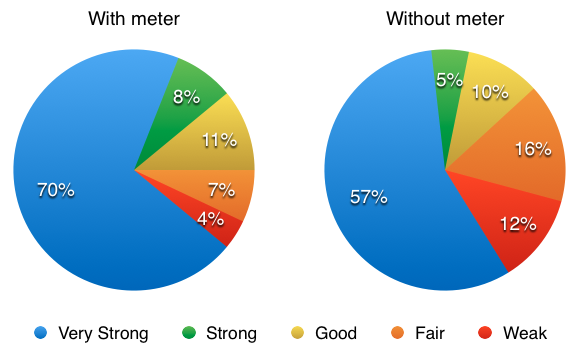
\includegraphics[width=\linewidth]{Images/results-str}
        \captionof{figure}{Pie charts of verdict frequencies}
        \label{fig:verdict}
      \end{minipage}
    \end{table}

    From the generated overview, a noticeable effect on the partial password strength can be observed. In order to test the null hypothesis $H_{0a}$, we performed a t-test on the normalised partial password strengths. The samples from the two groups of participants are considered independent and identically distributed, so we use the unpaired, two-sample, unequal variance test (Welch's t-test~\cite{t_test}) with two tails. As we previously mentioned, for this test we had decided (\emph{a priori}) to use a significance level of $\alpha = 0.01$.

    Judging from the results of this process, which is presented in Table~\ref{tab:t-test}, we observe that the t-statistic of the experimental data is over the critical value. We therefore \textbf{reject the null hypothesis $H_{0a}$ (with 99\% confidence) and claim that the partial password strength meter has a measurable positive effect in the strength of the created partial passwords}.

    \begin{table}[htpb]
      \centering
      \begin{tabular}{l r r}
      \toprule
      & \textbf{Meter} & \textbf{No Meter} \\
      \midrule
      \textbf{Mean $(\overline{X})$} & 86.2767 & 75.3703 \\
      \textbf{Variance ($\sigma^2$)} & 577.7259 & 1061.4647 \\
      \textbf{\# of Observations} & 100 & 100 \\
      \midrule
      \textbf{Hypothesised mean difference} & \multicolumn{2}{c}{0} \\
      \textbf{Degrees of freedom ($df$)} & \multicolumn{2}{c}{182} \\
      \textbf{t-statistic} & \multicolumn{2}{c}{2.6938} \\
      \textbf{$P(T\leq t)$ two-tail} & \multicolumn{2}{c}{0.0077} \\
      \textbf{t critical two-tail} & \multicolumn{2}{c}{2.6031} \\
      \bottomrule
      \end{tabular}
      \caption{t-Test: Two-Sample - Unequal Variances, $\alpha = 0.01$}
      \label{tab:t-test}
    \end{table}

    Apart from the main hypothesis that was tested, the answers in the study offer insight in various other aspects of partial passwords. Testing for differences between demographics indicated that there was no discernible variation in strength between men and women and neither age seemed to affect partial password strength. Participants aged 55+ had a 12\% higher than average score, but the population sample is small enough (8) that it can likely be statistical noise. Similarly, workers from India had a lower than average password strength (69.34), but the small sample (9) does not allow us to draw any conclusions.

    The experiment and control group displayed a similar distribution in their perceptions of their own password's resilience against partial attacks, both being in general more pessimistic than what the meter suggested (or would have suggested, in the case of the control group). This similar distribution in perceived strength, combined with the significant differences in the actual password strength leads to the control group displaying a slightly positive correlation (+0.225 factor) between perceived and actual strength, while the experiment group having practically no correlation at all (-0.076 factor). This comes as a surprise, considering that 60\% of the experiment group indicated that they did not believe the strength meter gave an incorrect score to their password, and only 19\% disagreed with the displayed score.\footnote{When values do not sum to 100\%, the difference exists in the \emph{Neutral} response of the scale.}

    A question in the survey concerned the methods subjects used to count the characters, when answering the partial password challenge; this is of particular interest, since it a unique feature that applies only to partial passwords. We discovered that the subjects' methods of counting the characters did not differ significantly between conditions, as shown in Figure~\ref{fig:counting-methods}. Mental counting appears as the main method of counting with 42\% of the total subjects reporting to use it, counting with fingers came second with 32\%, while counting while seeing the password came at a close third, with 26\% of participants.

    \begin{figure}[htpb]
      \centering
      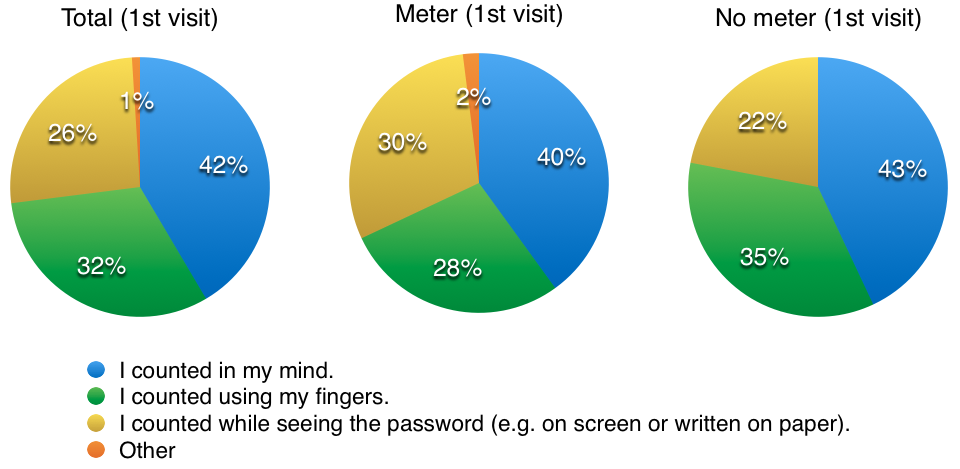
\includegraphics[width=\textwidth]{Images/counting}
      \caption{Counting methods for the partial password challenge}
      \label{fig:counting-methods}
    \end{figure}

    As this project lies at the intersection of computer security with HCI, it is important to examine the strength meter from a usability perspective, and the first questions in this survey were designed to help do so. Participants in the experiment group were asked to indicate their level of agreement on statements concerning the helpfulness of the password meter on creating stronger passwords, the importance of getting a high rating, the annoyance caused by it and their judgement of its correctness. Subjects in the control group were asked similar questions, but for strength meters in general; the exact wording of the statements can be found in Appendix~\ref{aps:survey_usability}, and the contingency table generated from them is displayed in Table~\ref{tab:beliefs}.

    \begin{table}[htpb]
      \centering
      \scriptsize
      \hspace*{-2cm}
      \begin{tabular}{p{3cm} rrrrrrrr}
        \toprule
         & \multicolumn{2}{c}{\textbf{Helpfulness}} & \multicolumn{2}{c}{\textbf{Importance}} & \multicolumn{2}{c}{\textbf{Annoyance}} & \multicolumn{2}{c}{\textbf{Incorrect results}} \\
        \textbf{Level of Agreement} & \textbf{Meter} & \textbf{No meter} & \textbf{Meter} & \textbf{No meter} & \textbf{Meter} & \textbf{No meter} & \textbf{Meter} & \textbf{No meter} \\
        \midrule
         \textbf{Strongly Agree} & 17 & 13 & 25 & 19 & 2 & 15 & 6 & 5 \\
         \textbf{Agree} & 46 & 52 & 44 & 31 & 5 & 20 & 13 & 22 \\
         \textbf{Neither Agree \newline or Disagree} & 20 & 14 & 16 & 24 & 11 & 7 & 21 & 27 \\
         \textbf{Disagree} & 13 & 18 & 9 & 21 & 40 & 41 & 42 & 40 \\
         \textbf{Strongly Disagree} & 4 & 3 & 6 & 5 & 42 & 17 & 18 & 6\\
        \bottomrule
      \end{tabular}
      \caption{Participants' beliefs about password meter}
      \label{tab:beliefs}
    \end{table}

    We can observe that the subjects in the \emph{Meter} condition had a generally positive experience with the partial password strength meter. 63\% of them reported that it helped them select a stronger password, with only 17\% claiming it did not help them, while the vast majority 80\% did not consider it annoying. Running omnibus (Pearson's $\chi^2$ goodness of fit~\cite{chi_sq}) tests between the groups, we discovered that a borderline significant difference ($p=0.048$) difference exists on how important a high score on the displayed strength meters is. Accounting for the bias introduced by the fact that object of the research was clear to the participants, we suggest not accepting this result as significant, as to avoid type I errors. A certain difference between the groups was observed in the annoyance caused by this vs password meters in general, with a probability $p=0.0000040 \ll \alpha = 0.05$. The margin is large enough for us to safely conclude that there is a substantial difference in that aspect, but we need to keep in mind that possible confusions between \emph{``password meter''} and \emph{``password policy''} might have influenced the results of the control group.


\section{Effect on partial password memorability}
  \label{sec:memorability}
  In this section, we detail the methodology followed while testing the $H_{0b}$ null hypothesis, and report our results, as well as other findings that emerged from the analysis of the collected data.

  \subsection{Methodology}
    \label{ssec:memorability_setup}
    Four days after each participant's completion of the task, they were sent an email informing them about a new, follow-up survey that they could return and complete. For the final part of the study, workers were compensated with 10 cents for attempting to login, while those who were able to remember their password and successfully login were granted a bonus of 22 cents, as advertised. This reward allocation method was used in order to give MTurk workers a monetary incentive to try and recall their passwords, as Ipeirotis discovered that one of their primary motivations is the financial compensation~\cite{mturk_demographic}. At the same time this allocation was fair, since workers who forgot their passwords were not presented with a survey and consequently spent less time on the HIT.

    Participants were asked to return to our website and answer a short survey, which was presented to them after a successful login using a partial password challenge. It was made clear to them (in the HIT instructions) that they would be able to complete the task regardless of their ability to recall their passwords, by clicking on a ``Forgot Password'' link, forfeiting the bonus. This was done in order to reassure them and encourage the participation of the subjects that had since forgotten their passwords \footnote{N.B. the HIT approval rate \% is an important metric in the MTurk platform, so workers generally avoid HITs they fear failing}. It is imperative to note here that during the first part of the study subjects \textbf{were informed} that they would need to remember their passwords for future use and asked to employ their usual methods for remembering and protecting an important password.

    From the 200 participants invited, 144 returned to complete the second part of the study. Those that succeeded in recalling their password were asked questions about the difficulty in recalling it, the method they used to remember it and (again) the method of counting the characters for the partial challenge. They were also asked how many unsuccessful attempts they made before logging in; this is something that can be measured server-side but it was not implemented and the work by Ur et al. indicated that workers were generally honest when answering those questions, with only 1.6\% found lying in their responses~\cite{strength_meter_effect}.

  \subsection{Results}
    \label{ssec:memorability_results}

    The analysis began similarly with the first stage, by counting and grouping the results in order to get an overview of the meter's effect; the values are presented in Table~\ref{tab:memorability}. We observe that participants from both conditions were equally likely to accept the return HIT, which is in agreement with our expectations and that there is a very slight increase in memorability for subjects in the \emph{Meter} condition.

    \begin{table}[htpb]
      \centering
      \begin{tabular}{l rrr}
      \toprule
      & \textbf{Meter} & \textbf{No meter} & \textbf{Total} \\
      \midrule
       \textbf{Remembered} & 52 & 47 & 99 \\
       \textbf{Forgot} & 24 & 21 & 45 \\
       \textbf{Returned} & 73 & 71 & 144 \\
       \textbf{Remembered \%} & 71.23 & 66.20 & 68.75 \\
      \bottomrule
      \end{tabular}
      \caption{Memorability of partial passwords}
      \label{tab:memorability}
    \end{table}

    In order to examine the null hypothesis $H_{0b}$, we performed an omnibus ($\chi^2$ goodness of fit~\cite{chi_sq}) test on the actual and expected values. The calculated probability was $p=0.51$, indicating that there is a high probability that the differences were simply statistical noise; we therefore claim that we did not observe a significant effect of the partial password strength meter on the memorability of partial passwords and \textbf{accept $H_{0b}$}.

    After examining the collected data, there are other interesting observations to be made. As shown in Table~\ref{tab:remember}\footnote{Sum of values is larger than the number of subjects that remembered their passwords, as they were asked to ``select all that apply''} (and the accompanying Figure~\ref{fig:remember}), the main method of remembering was memorising the password (67\%), with writing them down being the second most frequent way (21\%). Ur et al.'s findings were that 38.0\% of the participants that returned had stored their passwords, either electronically or on paper, a value that does not significantly differ from our data (32.7\%), reinforcing our belief in the validity of the collected data. The results of $\chi^2$ tests on our data determined that the proportion of participants using each method did not differ between conditions ($p=0.741$), an outcome that also is in agreement with their findings. Two users who selected the ``Other'' option reported sending an email containing the password to themselves and taking a photo of the password using their mobile phones. It is regrettable to notice that only a very small portion of subjects in our sample employ password management software (e.g. KeePass, LastPass, 1Password etc), which was one of the most common suggestions security experts offered with regard to best online security practices~\cite{security_practices_experts}.

    \begin{table}[htpb]
      \begin{minipage}[b]{0.42\linewidth}
        \centering
        \small
        \begin{tabular}{l r}
          \toprule
          \textbf{Method} & \textbf{Count} \\ \midrule
          \textbf{Memorised} & 74 \\
          \textbf{Wrote down} & 23 \\
          \textbf{Stored in file} & 5 \\
          \textbf{Password manager} & 5 \\
          \textbf{Other} & 3 \\ \bottomrule
        \end{tabular}
          \caption{Remembering methods}
          \label{tab:remember}
      \end{minipage}\hfill
      \begin{minipage}[b]{0.55\linewidth}
        \centering
        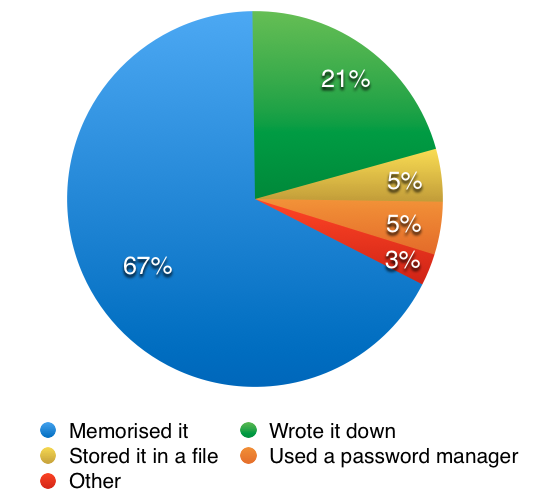
\includegraphics[width=\linewidth]{Images/remember-method}
        \captionof{figure}{Pie chart of remembering methods}
        \label{fig:remember}
      \end{minipage}
    \end{table}

    Because of the partial password setting of the study, we chose to examine changes in the ways participants used to count the characters between the first and second stage. As seen in Table~\ref{tab:counting_changes}, subjects who counted the characters in their minds or while seeing them did not significantly change their behaviour; 78.1\% and 80.6\% of them, respectively, reported using the same method between the two stages of the study. On the other hand, only 64.7\% of the subjects that counted using their fingers indicated that they used the same method the second time they logged in. From the workers that changed their way of counting, we observed that most switched to counting while seeing the password, with the ``changed'' users constituting the 34.2\% of the total number or subjects found using the method; the corresponding percentages were 21.9\% and 18.5\% for mental and finger counting. This behaviour can possibly be attributed to the subjects storing or writing the passwords down as a means to remember it - the coinciding numbers of those that somehow stored their password (36) with those that reported counting while seeing the password (38) further strengthen this assumption.


    \begin{table}[htpb]
      \centering
      \small
      \begin{tabular}{l rrr}
      \toprule
      \textbf{From/To} & \textbf{Mental} & \textbf{Fingers} & \textbf{Seeing pass} \\
      \midrule
       \textbf{Mental} & 25 & 2 & 5 \\
       \textbf{Fingers} & 4 & 22 & 8 \\
       \textbf{Seeing pass} & 3 & 3 & 25 \\
      \bottomrule
      \end{tabular}
      \caption{Changes in counting methods for partial password challenges}
      \label{tab:counting_changes}
    \end{table}

    % TODO: reset count-forgot correlation?
